\section{Gatling}

\subsection{Présentation de Gatling}

\subsubsection{Qu'est-ce que Gatling ?}

Gatling est un injecteur de charge open source, développé par Excilys et disponible depuis Janvier 2012.\\
Le but d'un injecteur de charge est d'effectuer des tests de charge sur une application web, en simulant l'activité des  utilisateurs et leur navigation à travers les différentes pages.\\

Les développeurs d'une telle application peuvent ainsi tester et vérifier la qualité de leur design et de leur implémentation en analysant la résistance de celle-ci à une utilisation simultanée par un grand nombre d'utilisateurs et met éventuellement en évidences les points chauds de leur application où une baisse de performances est observable, les aidant ainsi à le corriger, avant la mise en production.\\
Les rapports produits par Gatling constituent également une preuve concrète de la qualité du travail des développeurs pour leur hiérarchie ou leurs clients.


\subsubsection{Pourquoi avoir créé Gatling ?}

Gatling n'est pas le seul ni le premier injecteur de charge disponible sur le marché.\\
Il existe de nombreux concurrents :
\begin{itemize}
	\item JMeter
	\item LoadUI
	\item LoadRunner
	\item The Grinder
	\item etc\ldots \\
\end{itemize}

Cependant tous ces outils présentent différents inconvénients :
\begin{itemize}
	\item Certains sont payants, et la licence peut être très coûteuse (10000\$ dans le cas de LoadUI
	\item Certains sont codés dans d'autres langages que Java, compliquant leur compréhension ou leur debuggage par des développeurs Java
	\item Certains ne fonctionnent que sur Windows
	\item Enfin, leur performance ne permettent pas toujours de simuler des tests de charge intensifs (plusieurs milliers d'utilisateurs, parfois sur de longues durées)
	\item L'écriture de leur scénario de tests peut être complexe ou les scénarios peuvent être difficiles à maintenir\\
\end{itemize}

Gatling a donc été mis au point afin d'offrir une alternative, gratuite, à ces différentes solutions.

\subsubsection{Qu'est ce qui différencie Gatling de ces autres solutions ?}

Le modèle d'\textit{acteurs} sur lequel repose Gatling ainsi que son utilisation des communications asynchrones font que Gatling est peu gourmand en ressources (CPU ou mémoire).
JMeter, par exemple, exigera une machine très performante voire d'un ensemble de machines pour réaliser des tests que Gatling peut effectuer sur une machine aux performances modérées.\\

Une autre différence importante entre Gatling et ses concurrents est le format des scénarios de tests (ou \textit{simulations}).\\
Alors que de nombreux outils utilisent un fichier au format XML afin de décrire leur simulations, ce qui les rend plus difficilement manipulables sans passer par l'outil et également plus difficiles à maintenir, les simulations de Gatling sont écrits sous forme de code Scala, simples à modifier, à mettre à jour et à intégrer au reste du projet (dans le cadre d'un système de contrôle de version par exemple).

\subsection{Technologies utilisées}

\subsubsection{Scala}

Scala est un langage de programmation multi-paradigme (objet et fonctionnel).\\

La principale différence entre Scala et d'autres langages fonctionnels tels que OCaml, Haskell ou Lisp est qu'il est conçu pour fonctionner sur une JVM (machine virtuelle Java).\\
 Ceci permet à n'importe quel code Scala d'utiliser du code Java existant sans manipulation particulière, offrant ainsi aux développeurs la possibilité d'utiliser toutes les librairies et frameworks écrits en Java. Il est également tout à fait possible d'intégrer d'utiliser du code Scala dans du code Scala.\\

Bien que moins répandu que Java, Scala est un langage qui prend petit à petit de l'ampleur et est déjà au coeur de certaines applications parmi les exigeantes (le moteur de gestion des tweets de Twitter est codé en Scala).

\subsubsection{Akka}

Akka est un toolkit permet de réaliser simplement des applications concurrentes et distribuées.\\
Ceci est permis par le modèle de communication utilisé par Akka basé sur les \textbf{acteurs}.\\

Dans le cas de Gatling, plutôt que de représenter chaque utilisateur par un thread, il est représenté par un acteur.

Chaque acteur dispose d'une \textbf{mailbox}, stockant les messages envoyés par les autres acteurs du système. Lorsqu'un acteur a reçu des message et que ceux-ci doivent être traités, un thread se charge alors de \og prendre en charge \fg{} cet acteur et ses messages le temps de les traiter et redevient par la suite disponible pour un autre acteur. Il s'agit donc d'un modèle asynchrone.

Par exemple, là où un modèle 1 utilisateur = 1 thread aurait donc nécessité la création de 1000 threads pour 1000 utilisateurs, une application s'appuyant sur le modèle d'acteur d'Akka  peut très bien se contenter de créer quelques dizaines de threads pour gérer ces mêmes 1000 utilisateurs.\\

Akka dispose également de fonctionnalités avancés de tolérance aux pannes, de supervision des acteurs  par d'autres acteurs (via une hiérarchisation de ceux-ci), d'acteurs distribués\ldots

Akka est par exemple au cœur du \textit{Play! Framework}, framework destinée aux applications web et écrit en Scala.\\

Une des raisons ayant poussé le choix de Scala pour Gatling est qu'Akka est lui-même développé dans ce langage et que celui-ci est le plus adapté pour développer des applications reposant sur Akka.
 
\subsubsection{Netty \& Async HTTP Handler}

Async HTTP Handler est un client HTTP reposant sur le moteur Netty qui permet de gérer l'envoi de requêtes (et le traitement des réponses) HTTP de manière asynchrone, complétant ainsi le caractère asynchrone d'Akka, ce qui permet à Gatling de disposer d'un moteur intégralement asynchrone.

\subsubsection{Metrics}

Metrics est une librairie développée par Codahale et créée à l'origine pour le réseau social Yammer.\\

Metrics offre un panel de métriques (compteurs, histogrammes, taux par seconde\ldots) qu'il est possible d'ajouter au code d'une application afin de mesurer certains évènements.\\
Metrics offre également la possibilité d'exporter ces métriques vers des outils de reporting tels que Graphite ou Ganglia, offrant ainsi une solution complète de monitoring de l'application cible.
\subsection{Architecture de Gatling}

\begin{center}
	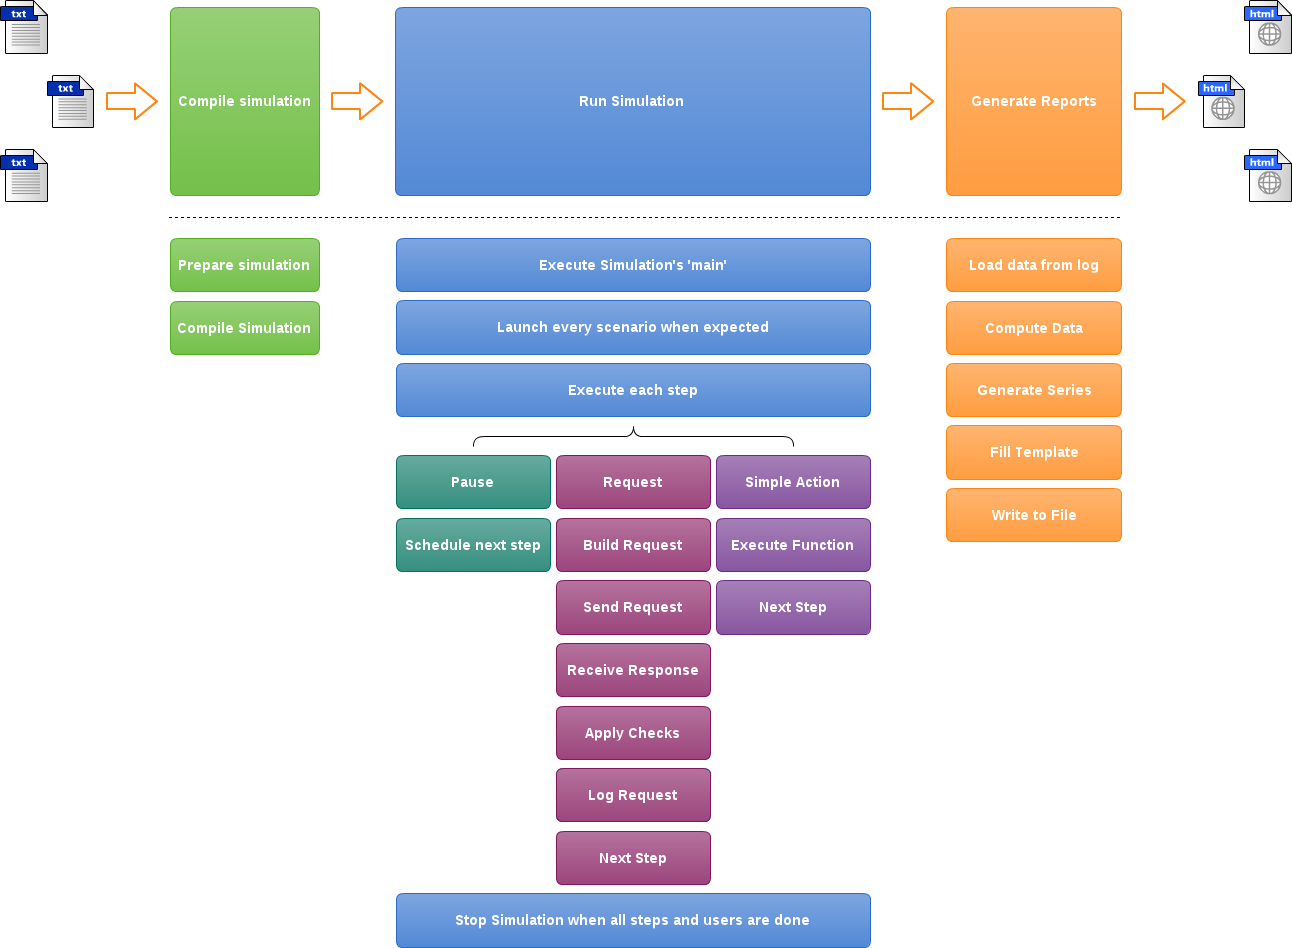
\includegraphics[scale=0.3]{gatling-process.png}
\end{center}

\subsection{Encadrement du projet Gatling et méthodes de travail}

Ma participation au projet Gatling a été encadrée par Stéphane LANDELLE, \textit{Product Owner} de Gatling et qui le développe actuellement à plein temps.\\
En tant que \textit{Product Owner}, Stéphane décide des fonctionnalités que nous devions ajouter à Gatling. Quand nous avons une piste pour implémenter une des fonctionnalités souhaitées, nous vérifions avec lui que cette piste lui convient et le cas échéant, nous commencons à l'implémenter.\\
Une fois l'implémentation achevée et testée, nous vérifions la qualité du code avant d'intégrer définitivement la fonctionnalité à Gatling.
\subsection{Fonctionnalitées réalisées ou en cours de réalisation}

\subsubsection{Monitoring c\^oté serveur}

Actuellement, les mesures prises par Gatling ne concernent que ce qu'un utilisateur de l'application observerait : le temps que met une page web à répondre ou tout simplement si celle répond ou non.\\
La première fonctionnalité que Stéphane souhaitait intégrer à Gatling est le monitoring de l'application testée, c\^oté serveur.\\

Ce choix était motivé par deux raisons :
\begin{itemize}
	\item Bien qu'étant open source (et donc sans volonté de réaliser de profits par le biais de Gatling), Gatling reste en concurrence avec d'autres produits gratuits ou payants et plusieurs produits payants proposent du monitoring c\^oté serveur ou comptent en intégrer dans un futur proche. Intégrer du monitoring c\^oté serveur  dans Gatling permettrait donc à celui-ci de ne pas prendre de retard sur la concurrence
	\item Monitorer l'application testée permettrait d'obtenir de précieuses informations sur le comportement de l'application durant le test que ça soit en terme d'utilisation CPU, de mémoire, d'activité des bases de données\ldots En recoupant ces informations avec celles déjà existantes, cela permettrait d'obtenir des rapports encore plus pertinents : On pourrait observer par exemple que, lors d'une baisse de performances de l'application, l'activité CPU explose ou la mémoire utilisée par l'application augmente fortement, ce qui pourrait mettre les développeurs de l'application sur la piste d'un problème dans l'implémentation.\\
\end{itemize}

J'ai donc, avec mes collègues, exploré les solutions possibles pour apporter cette fonctionnalité à Gatling.\\

Cela nous a très rapidement conduit à étudier JMX (Java Management Extensions).\\
JMX est une technologie disponible dans n'importe quel JDK standard qui offre la possibilité de créer des classes (les \textit{MBeans} gérant un ensemble de statistiques et de pouvoir exposer celle sur le réseau par le biais de protocoles de type RMI (Remote Method Invocation). Plusieurs MBeans sont d'ailleurs disponibles dans l'API standard Java, afin de monitorer le fonctionnement de la JVM (mémoire utilisée, statistiques sur le garbage collector\ldots).\\
JMX étant la solution la plus utilisée pour exposer des statistiques d'une application au monde éxterieur, il nous a semblé évident que le monitoring c\^oté serveur passerait par l'exploitation de JMX.\\

Deux problèmes se posaient cependant avec JMX : 
\begin{itemize}
	\item Comment gérer efficacement la remontée  de plusieurs dizaines, voire centaines de statistiques via JMX, le tout restant configurable par un utilisateur de Gatling ?
	\item JMX présente de potentiels problèmes de performance, de par son utilisation du protocole RMI. Si des nombreuses statistiques sont remontées et qu'il y a donc une forte activité du c\^oté de RMI, ne risque-t-on pas d'impacter, éventuellement de manière importante, les performances de l'application dont on cherche justement à évaluer les performances ?
\end{itemize}

Cela nous a donc conduit à rechercher des outils existants permettant de régler ces problèmes.\\
Le premier problème est en mesure d'être résolu grâce à l'outil Jmxtrans, spécialement conçu pour simplifier le requêtage répété de nombreux MBeans.\\
Le deuxième peut \^etre résolu en utilisant un agen Java. Un agent est un éxécutable Java venant se greffer sur une JVM afin d'interagir avec le code s'éxécutant sur celle-ci. Le problème de performance était ainsi reglé car, au lieu de faire appel aux MBeans à requ\^eter à travers RMI, la requ\^ete est directement effectuée sur les MBeans en local, au sein même de la JVM.\\

Nous avons alors créé plusieurs programmes afin de tester chacune des solutions, avec des résultats encourageants.\\
Malgré tout, d'autres choix techniques importants se posaient qui nécessiteraient un arbitrage de Stéphane et, étant donné que d'autres fonctionnalités devaient \^etre rapidement implémentées, nous avons pour l'instant laissé de c\^oté le monitoring c\^oté serveur afin de se concentrer sur ces autres fonctionnalités.

\subsubsection{Support de DataWriters optionnels}

Les DataWriters sont les classes de Gatling qui recoivent les résultats des requêtes effectuées et qui sont en charge de les traiter.\\
Deux DataWriters sont présents en standard dans Gatling : 
\begin{itemize}
	\item ConsoleDataWriter, en charge d'afficher régulièrement sur la console l'état d'avancement du test de charge : durée écoulée, nombres d'utilisateurs actifs, nombre de requêtes effectuées pour chacune des requêtes du scénario\ldots
	\item FileDataWriter, en charge d'écrire les résultats des requêtes dans un fichier de log afin qu'il puisse analysés par la suite pour produire le rapport de test.\\
\end{itemize}

Le besoin se faisait sentir de pouvoir supporter des DataWriters optionnels, notamment pour l'intégration de Metrics.\\
Etant donné que chaque DataWriter est un acteur Akka, j'ai retravaillé le code en charge du dispatch des résultats des requêtes aux différents DataWriters.\\
Là le code existant envoyait explicitement aux deux DataWriters le résultat des requêtes, j'ai mis en place un routeur\footnote{http://doc.akka.io/docs/akka/2.0.3/scala/routing.html} Akka,  en charge de renvoyer un message à l'ensemble de ses acteurs routés à qui je fournis la liste de tous les DataWriters actifs (gérés par un fichier de configuration). 
\subsubsection{Intégration Jenkins}

L'ajout d'une intégration de Gatling au serveur d'intégration continue Jenkins est motivée par l'interêt que peut avoir des tests de charge réguliers sur une application en cours de développement.\\
En effet, en exécutant à chaque build un test de charge (mis à jour pour tester les nouvelles fonctionnalités ajoutées par le code mis à jour) permet de surveiller constamment les performances de l'application et d'observer l'impact des nouveaux ajouts sur les fonctionnalités pré-existantes.\\

Deux voies ont été envisagées pour réaliser cette intégration, en se basant sur le système de \textit{plugins} de Jenkins : 
\begin{itemize}
	\item Utiliser le HTML Publisher Plugin, afin de publier automatiquement les résultats des simulations de Gatling(qui prennent la forme d'une page HTML)
	\item Utiliser le Performance Plugin, et lui fournir les données en entrée pour qu'il puisse générer ses graphiques 
\end{itemize}

La solution se basant sur le HTML Publisher Plugin n'a pas été retenue car l'intégration qui en résultait n'était pas assez poussée (on disposait tout au mieux d'un lien vers la pages des résultats).\\

La solution se basant sur le Performance Plugin a donc été privilégiée, car les fonctionnalités offertes par ce plugin sont bien supérieures,entre autres : 
\begin{itemize}
	\item Intégration plus poussée de la page de résultats des simulations au sein de l'interface de Jenkins
	\item Graphiques montrant l'évolution des résultats des simulations de build en build\\
\end{itemize}

Le problème auquel j'ai été confronté est que le Performance Plugin ne supporte que deux formats en entrée : le format de logs de Junit et celui de JMeter, et le format des logs de Gatling n'était compatible avec aucun d'entre eux.
En effet, les formats de logs de Junit et de JMeter sont tous deux basés sur XML, alors que Gatling écrit ses résultats au format TSV (\textit{tab$-$separated values}).\\

Une première solution à ce problème a été proposée par un développeur de Gatling : modifier le Performance Plugin (qui est open-source) afin qu'il supporte le format des logs de Gatling.\\
Cependant, cette solution n'était pas pérenne, car elle reposait sur une version \og alternative \fg{} du Performance Plugin, et tous les utilisateurs de Gatling souhaitant bénéficier de cette intégration auraient dû installer ce nouveau plugin depuis les sources, alors que le Performance Plugin de base peut \^etre installé en quelques clics depuis Jenkins. L'ajout pourrait également être proposé aux développeurs en charge du Performance Plugin, mais rien ne garantit qu'ils auraient accepté d'intégrer cette ajout, surtout que Gatling reste un outil relativement jeune.\\

La solution a été de prendre le problème dans l'autre sens : plutôt que de forcer le  Performance Plugin à pouvoir lire le format de logs de Gatling, c'est à Gatling d'écrire ses logs dans un format supporté par le Performance Plugin.\\
Comme évoqué précedemment, deux formats sont actuellement supportés :
\begin{itemize}
	\item Le format de logs de Junit
	\item Le format de logs de JMeter
\end{itemize}
J'ai étudié en détail ces deux formats, afin de définir celui qui sera le plus adapté mais également le plus simple à écrire.\\

Le format de logs de Junit a été rapidement écarté, car il ne correspond absolument pas aux besoins de Gatling : de nombreux informations non pertinentes dans le cadre d'un test de charge doivent être indiquées et peu d'informations peuvent être précisées concernant les tests à proprement parler.\\ Plus simplement, le format de logs de Junit est uniquement pensé\ldots pour des logs de tests unitaires Junit.\\

Mon choix s'est donc porté sur le format de logs de JMeter. Pour les besoins de Gatling, le format est extrêmement simple :
\begin{itemize}
	\item La déclaration XML
	\item Le résultat de chaque requête est représenté par un élements ayant comme tag \textit{httpSample}, dont les détails sont représentés par une série d'attributs
\end{itemize}
Gérer l'écriture des logs dans ce nouveau format n'a pas posé de problème particulier,étant donné que toutes les informations nécessaires étaient accessibles et qu'assurer un formatage correct des balises fut suffisant.\\

Les premiers tests furent très convaincants : le format était respecté, les logs étaient correctement traités par le Performance Plugin générait correctement les graphiques.\\
Mais des test complémentaires demandés par Stéphane démontrèrent que le Performance Plugin n'est pas une solution viable quand il est utilisé avec Gatling :  la combinaison d'Akka et de Netty permettant d'effectuer avec des ressources modestes des tests de charge avec plusieurs milliers d'utilisateurs, les logs des simulation ont tendance à attendre rapidement des tailles de plusieurs dizaines de méga-octets.\\
Les tests initiaux ne portaient que sur des simulations courtes avec peu d'utilisateurs (200 utilisateurs pendant 3 minutes environ). Mais un test avec 8000 utilisateurs pendant 15 minutes, générant un log de simulation d'une cinquaintaine de méga-octets, ont montré les limites du Performance Plugin : la génération des graphiques est beaucoup plus lente et l'affichage de résultats détaillés bloquait Jenkins pendant plusieurs dizaines de secondes.\\[1cm]

Étant donné que les solutions se basant sur des plugins Jenkins existants se sont toutes avérées être des impasses, la décision a été prise de créer directement un plugin  à Gatling.\\
La solution se basant sur le Performance Plugin étant abandonné, il n'est donc plus nécessaire de se baser sur le format JTL et le nouveau plugin va plutôt se baser sur les données déjà produites par Gatling.\\

Ce nouveau plugin offrira également plus de fonctionnalités que le Performance Plugin :
\begin{itemize}
	\item Le Performance Plugin permet de faire échouer une build ou de considérer comme instable en fonction à partir d'un certain pourcentage d'erreurs. Le nouveau plugin proposera plus de critères : temps de réponse moyen, temps de réponse maximal,95/99\up{èmes} percentiles sur le temps de réponse\ldots
	\item Les graphiques fournis par le nouveau plugin seront plus nombreux et plus détaillés\\
\end{itemize}

Le plugin est actuellement en cours d'écriture et sera terminé courant septembre, afin qu'il puisse \^etre intégré à la version 1.3 de Gatling, la prochaine version stable. 
\subsubsection{Ajout de métriques en temps réel à Gatling}

Les rapports créés par Gatling détaillant les résultats du test de charge sont très complets, mais ne peuvent être fournis qu'une fois le test terminé.Plusieurs utilisateurs de Gatling ont fait part de leur interêt pour une solution permettant d'avoir des résultats en temps réel, en se basant notamment sur des solutions populaires de monitoring telles que Graphite ou Ganglia.\\
La demande pour cette fonctionnalité ayant été assez forte, Stéphane a décidé que cette fonctionnalité serait implémentée.\\

Plusieurs pistes et librairies ont été envisagées mais la solution retenue a été l'intégration de la librairie Metrics\footnote{http://metrics.codahale.com} écrite par Codahale au sein de Gatling.\\

Deux problèmes ont cependant compliqué l'intégration \og directe \fg{}  de Metrics.\\

Tous les métriques proposées par \textit{thread-safe} et donc accessibles en toute sécurité par plusieurs threads simultanément, mais dans le cadre de Gatling et de l'utilisation d'Akka, un seul thread accéderait aux métriques à un instant $T$.\\
De plus rendre du code Java \textit{thread-safe} passe par l'utilisation de la synchronisations et par la prise et le rendu de verrous sur un objet, ce qui impacte les performances. les métriques étant mise à jour à chaque requête terminée, on arrive rapidement à plusieurs milliers de mises à jour par seconde et l'impact de la synchronisation sur les performances risquait de se faire sentir.\\

L'autre problème posé par Metrics est que nous avions besoin que certaines métriques soit calculées uniquement sur un intervalle d'une seconde, ce qui impliquait que les valeurs stockées par les métriques soient réinitialisés à chaque seconde, ce qui n'était pas proposé par les métriques par défaut de Metrics.\\  

J'ai donc dû réimplementer certaines métriques afin que celles-ci ne soient plus thread-safe mais qu'elles soient en contrepartie plus performantes. J'ai également dû implémenter des métriques dont les valeurs sont réinitialisés à chaque seconde.\\
Ces modifications ont conduit à réimplementer une bonne partie de l'architecture de Metrics car certains choix d'implémentations de Metrics (visibilité \textit{default} des classes, classes internes essentielles privées\ldots) rendent difficile une extension simple des fonctionnalités de Metrics (Metrics est en quelque sorte conçu pour être utilisé \og tel quel \fg{}).  \\

Le schéma ci-dessous décrit plus en détail la gestion des résultats des requêtes par mon intégration de Metrics à Gatling : 
\begin{itemize}
	\item Quand une requête termine, un objet RequestRecord contenant les résultats de la requête (temps mis pour éxécuter la requête, nom de la requête concernée dans la simulation, status OK/KO\ldots) est produit et transmis aux DataWriters, chargés de traiter ce RequestRecord.
	\item MetricsDataWriter est le point d'entrée du RequestRecord. Cette classe gère une Map associant une requête (via son nom) à un acteur Akka,RequestMetrics, en charge de conserver les métriques propres à cette requête et de les mettre à jour
	\item 	MetricsDataWriter ausculte le RequestRecord afin d'obtenir le nom de la requête et transmet le RequestRecord à l'instance RequestMetrics correspondante
	\item L'instance de RequestMetrics qui a reçu le RequestRecord le traite et met à jour les métriques qui doivent l'être.\\
\end{itemize}
\newpage
\begin{figure}[h!]
	\centering
		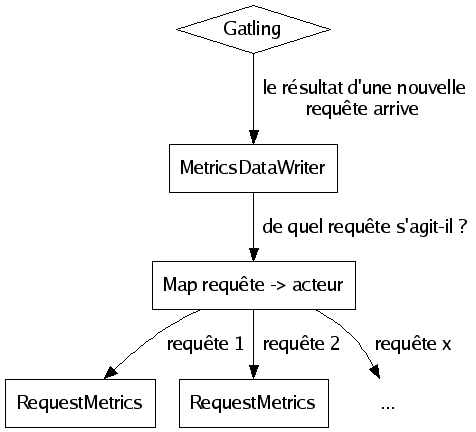
\includegraphics[scale=0.5]{metrics.png}
	\caption{Dispatch d'un résultat de requête}
\end{figure}

Actuellement, seul Graphite est supporté pour l'export des métriques, mais le support de Ganglia est envisagé si suffisament d'utilisateurs sont interessés.\\
L'intégration de Metrics ayant été finalisée et acceptée par Stéphane, elle est déjà disponible dans la version de développement et sera présente dans la prochaine version stable.